%==============================================================================
\chapter{Experimental Evaluations}\label{chap:experiments}
% Avaliação preliminar para a qualificação
%==============================================================================

In this chapter we present the research questions and hypotheses investigated during the evaluation of our proposal, in addition to the experimental design adopted and its conduct.
The preliminary evaluation is presented in Section \ref{sec_experiments:preliminaryEval} and the final evaluation in Section \ref{sec_experiments:finalEval}.
The chapter's lessons are presented in Section \ref{sec_experiments:lessons}

%------------------------------------------------------------------------------
\section{Preliminary Evaluation} 
\label{sec_experiments:preliminaryEval}
%------------------------------------------------------------------------------

This Section presents all the planning, conduction, discussion of the results obtained, threats to the study and the conclusions regarding the preliminary evaluation carried out to evaluate a stable prototype of the developed tool.

%######################################################
\subsection{Planning}
\label{ssec_experiments:preliminary_planning}
%######################################################

This preliminary evaluation was carried out from the replication of the experimental protocol performed in a previous study \cite{Lopes:2019} and aims to obtain evidence from the comparison of two approaches for modeling relational databases, one graphical and the other textual.

The treatments identified were:
\begin{enumerate} [label=\roman*]
    \item. Control treatment: the brModelo tool (graphical approach), and;
    \item. Experimental treatment: the ERtext tool (textual approach).
\end{enumerate}
The purpose of this replication is to evaluate the feasibility of using a textual approach to support the teaching-learning process of conceptual modeling of relational databases.

\textbf{Context:}
The context of the experiment is characterized according to four dimensions:
\begin{enumerate}[label=\roman*]
    \item. Process: an \textit{in-vitro} approach was used, since the tasks were performed under controlled conditions.
    %In software engineering, most \textit{in-vitro} experiments are executed in universities or among selected groups of a software development organization \cite{Travassos:2003}.
    \item. Subjects: undergrad students in Computer Science (CS) and SE programs.
    \item. Reality: the experiment addressed a real problem, \textit{i.e.} the difference in the effort spent of subjects in the conceptual modeling of relational databases. 
    %the artifacts quality produced and the subjects Perceived Usefulness (PU) using both approaches.
    \item. Generality: this evaluation is inserted in a specific context, involving database modeling students.
    However, the general ideas of this experiment can be replicated in another set of subjects, approaches or DSLs that support database designing.
\end{enumerate}

\textbf{Research Questions (RQs):}
For the discussion of the controlled experiment results, we decided to formulate four RQs that were related to the activities performed in the protocol execution.
\begin{itemize}
    \item \textbf{RQ1.} Which approach requires the most effort spent on average during the modeling activity?
    \item \textbf{RQ2.} What is the quality level of the models produced using the graphical and textual approaches?
    \item \textbf{RQ3.} What is the subjects perception regarding the Perceived Ease of Use (PEoU) and Perceived Usefulness (PU) of the proposed DSL?
    \item \textbf{RQ4.} What is the subjects assessment in relation to the representation of the ER modeling builders supported in the proposed DSL?
\end{itemize}

\textbf{Hypotheses Formulation:} 
The first two RQs were taken into account. Regarding to \textbf{RQ1.} 
%the average effort spent required using each approach, our scientific hypotheses are as follows:
% we defined a two-sided hypotheses that measure the average effort spent between textual and graphical approaches during conceptual modeling. State the null (no difference) $H_0 : \mu Time_T = \mu Time_G$ and alternative (significant difference) $H_a : \mu Time_T \neq Time_G$ hypotheses.
\begin{itemize}
    \item \textbf{Null hypothesis:} $H_0 : \mu Time_T = \mu Time_G$: There is no difference in average effort spent measure between textual and graphical approaches during conceptual modeling.
    \item \textbf{Alternative hypothesis:} $H_{1} : \mu Time_T \neq \mu Time_G$: There is a significant difference in average effort spent measure between textual and graphical approaches during conceptual modeling.
\end{itemize}
Regarding to \textbf{RQ2.} 
%the modeling effectiveness using each approach, our hypotheses are as follows:
in the same way we stated a two-sided hypotheses that measure the modeling effectiveness between textual and graphical approaches during conceptual modeling.
% The null (no difference) and alternative (significant difference) hypotheses are, respectively: 
% $H_0 : \mu Effectiveness_T = \mu Effectiveness_G$ and 
% $H_a : \mu Effectiveness_T \neq \mu Effectiveness_G$.
\begin{itemize}
    \item \textbf{Null hypothesis:} $H_0 : \mu Effectiveness_T = \mu Effectiveness_G$: There is no difference in effectiveness measure between textual and graphical approaches during conceptual modeling.
    \item \textbf{Alternative hypothesis:} $H_{1} : \mu Effectiveness_T \neq \mu Effectiveness_G$: There is a significant difference in effectiveness measure between textual and graphical approaches during conceptual modeling.
\end{itemize}

\textbf{Statistical Methods:} Unlike the first experiment, this replication included a change in the statistical methods adopted.
Previously, the Shapiro-Wilk normality test and the paired T-test for dependent samples were used.
This was because the sample was smaller (27) than 30 elements.
However, for samples equal to or greater than this quantity, alternative tests are recommended~\cite{Triola:2018}.

For the effort we chose the Kolmogorov-Smirnov test to verify normality, and the Wilcoxon Signed-Rank test for paired samples to investigate the hypotheses using the time spent metric.
For the effectiveness tests, the same statistical methods were adopted, but instead of using the time spent metric, another measure was necessary.
Thus, the F1 calculations were performed, which is derived from harmonic mean of \textit{Precision} and \textit{Recall} metrics, for each of the models produced in both approaches.
The F1 calculation \cite{Derczynski:2016} takes into account variables known as \textit{True Positives}, \textit{False Positives} and \textit{False Negatives}.
\begin{description}
% \begin{inparadesc}
    \item \textbf{\textit{True Positives (TP)}}: Amount of elements correctly modeled using the approach.
    \item \textbf{\textit{False Positives (FP)}}: Amount of elements incorrectly modeled using the approach. 
    \item \textbf{\textit{False Negatives (FN)}}: Amount of elements not modeled using the approach.
% \end{inparadesc}
\end{description}
From the variables identification it is then possible to calculate the \textit{Precision}, \textit{Recall} and \textit{F1} of each model according to these formulas:
\begin{description}
    \item \textbf{\textit{Precision (PR)}}: $\frac{TP}{TP~+~FP}$ 
    \hfill 
    \textbf{\textit{Recall (RE)}}:$\frac{TP}{TP~+~FN}$
    \hfill
    \textbf{\textit{F1-Score (F1)}}: $\frac{2~*~(PR~*~ RE)}{PR~+~RE}$
\end{description}

\textbf{Experiment Design:} Finally, the design of the controlled experiment performed is presented in Figure \ref{fig:designExp}. 
We followed the design of one factor with two treatments, where we blocking, balancing and randomizing the subjects, which carried out both treatments, featuring a paired comparison design.

\begin{figure}[!htb]
    \centering
    

\tikzset{every picture/.style={line width=0.75pt}} %set default line width to 0.75pt        

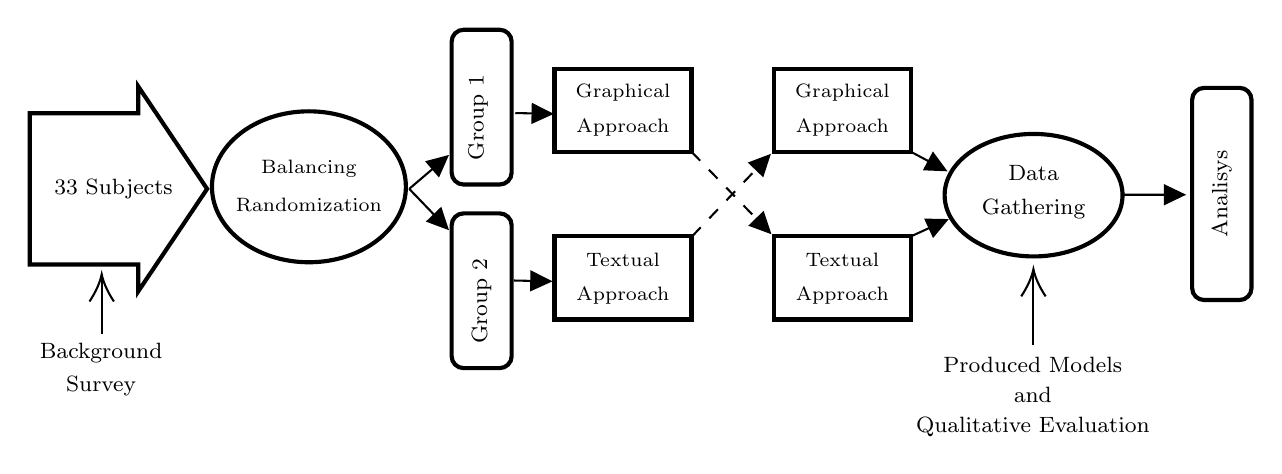
\begin{tikzpicture}[x=0.9pt,y=0.9pt,yscale=-1,xscale=1]
%uncomment if require: \path (0,327); %set diagram left start at 0, and has height of 327


%Shape: Ellipse [id:dp633810982278807] 
\draw  [line width=1.5]  (84.73,72.26) .. controls (84.73,55.52) and (102.16,41.96) .. (123.66,41.96) .. controls (145.16,41.96) and (162.59,55.52) .. (162.59,72.26) .. controls (162.59,88.99) and (145.16,102.56) .. (123.66,102.56) .. controls (102.16,102.56) and (84.73,88.99) .. (84.73,72.26) -- cycle ;



%Shape: Ellipse [id:dp7904221795411808] 
\draw  [line width=1.5]  (378.89,75.63) .. controls (378.89,62.05) and (394.88,51.04) .. (414.61,51.04) .. controls (434.33,51.04) and (450.32,62.05) .. (450.32,75.63) .. controls (450.32,89.21) and (434.33,100.22) .. (414.61,100.22) .. controls (394.88,100.22) and (378.89,89.21) .. (378.89,75.63) -- cycle ;

%Rounded Rect [id:dp5302697683495847] 
\draw  [line width=1.5]  (180.95,87.75) .. controls (180.95,85.09) and (183.11,82.93) .. (185.77,82.93) -- (200.23,82.93) .. controls (202.9,82.93) and (205.06,85.09) .. (205.06,87.75) -- (205.06,140.25) .. controls (205.06,142.91) and (202.9,145.07) .. (200.23,145.07) -- (185.77,145.07) .. controls (183.11,145.07) and (180.95,142.91) .. (180.95,140.25) -- cycle ;
%Rounded Rect [id:dp9616486966995694] 
\draw  [line width=1.5]  (180.95,14.03) .. controls (180.95,11.37) and (183.11,9.21) .. (185.77,9.21) -- (200.23,9.21) .. controls (202.9,9.21) and (205.06,11.37) .. (205.06,14.03) -- (205.06,66.52) .. controls (205.06,69.19) and (202.9,71.35) .. (200.23,71.35) -- (185.77,71.35) .. controls (183.11,71.35) and (180.95,69.19) .. (180.95,66.52) -- cycle ;

%Shape: Rectangle [id:dp03801896284105699] 
\draw  [line width=1.5]  (222.23,24.87) -- (277.28,24.87) -- (277.28,58.21) -- (222.23,58.21) -- cycle ;
%Straight Lines [id:da1799424135415575] 
\draw    (163.93,73.09) -- (177.61,61.43) ;
\draw [shift={(179.89,59.48)}, rotate = 499.54] [fill={rgb, 255:red, 0; green, 0; blue, 0 }  ][line width=0.08]  [draw opacity=0] (8.93,-4.29) -- (0,0) -- (8.93,4.29) -- cycle    ;
%Straight Lines [id:da17029537209985257] 
\draw    (163.93,73.09) -- (177.81,87.53) ;
\draw [shift={(179.89,89.69)}, rotate = 226.13] [fill={rgb, 255:red, 0; green, 0; blue, 0 }  ][line width=0.08]  [draw opacity=0] (8.93,-4.29) -- (0,0) -- (8.93,4.29) -- cycle    ;
%Straight Lines [id:da39402523544663426] 
\draw  [dash pattern={on 4.5pt off 4.5pt}]  (277.5,92.15) -- (307.06,61.21) ;
\draw [shift={(309.13,59.04)}, rotate = 493.69] [fill={rgb, 255:red, 0; green, 0; blue, 0 }  ][line width=0.08]  [draw opacity=0] (8.93,-4.29) -- (0,0) -- (8.93,4.29) -- cycle    ;
%Straight Lines [id:da7992081880522388] 
\draw  [dash pattern={on 4.5pt off 4.5pt}]  (277.28,58.21) -- (307.27,89.16) ;
\draw [shift={(309.35,91.31)}, rotate = 225.9] [fill={rgb, 255:red, 0; green, 0; blue, 0 }  ][line width=0.08]  [draw opacity=0] (8.93,-4.29) -- (0,0) -- (8.93,4.29) -- cycle    ;
%Right Arrow [id:dp3913444800583221] 
\draw  [line width=1.5]  (11.57,42.74) -- (55.14,42.74) -- (55.14,31.99) -- (82.78,73.11) -- (55.14,114.23) -- (55.14,103.49) -- (11.57,103.49) -- cycle ;
%Shape: Rectangle [id:dp003852149638719382] 
\draw  [line width=1.5]  (310.31,24.87) -- (365.36,24.87) -- (365.36,58.21) -- (310.31,58.21) -- cycle ;
%Shape: Rectangle [id:dp0126542660109914] 
\draw  [line width=1.5]  (310.31,92.18) -- (365.36,92.18) -- (365.36,125.52) -- (310.31,125.52) -- cycle ;
%Shape: Rectangle [id:dp4954877903085966] 
\draw  [line width=1.5]  (222.23,92.18) -- (277.28,92.18) -- (277.28,125.52) -- (222.23,125.52) -- cycle ;
%Straight Lines [id:da3442884963113835] 
\draw    (365.36,58.21) -- (377.4,64.63) ;
\draw [shift={(380.04,66.05)}, rotate = 208.07999999999998] [fill={rgb, 255:red, 0; green, 0; blue, 0 }  ][line width=0.08]  [draw opacity=0] (8.93,-4.29) -- (0,0) -- (8.93,4.29) -- cycle    ;
%Straight Lines [id:da6883068419855551] 
\draw    (365.36,92.18) -- (377.84,86.46) ;
\draw [shift={(380.57,85.22)}, rotate = 515.4100000000001] [fill={rgb, 255:red, 0; green, 0; blue, 0 }  ][line width=0.08]  [draw opacity=0] (8.93,-4.29) -- (0,0) -- (8.93,4.29) -- cycle    ;
%Rounded Rect [id:dp5928061300931144] 
\draw  [line width=1.5]  (478.27,37.32) .. controls (478.27,34.68) and (480.41,32.55) .. (483.04,32.55) -- (497.34,32.55) .. controls (499.97,32.55) and (502.1,34.68) .. (502.1,37.32) -- (502.1,112.96) .. controls (502.1,115.59) and (499.97,117.72) .. (497.34,117.72) -- (483.04,117.72) .. controls (480.41,117.72) and (478.27,115.59) .. (478.27,112.96) -- cycle ;

%Straight Lines [id:da6932528701926595] 
\draw    (450.32,75.46) -- (472.85,75.45) ;
\draw [shift={(475.85,75.45)}, rotate = 539.96] [fill={rgb, 255:red, 0; green, 0; blue, 0 }  ][line width=0.08]  [draw opacity=0] (8.93,-4.29) -- (0,0) -- (8.93,4.29) -- cycle    ;
%Straight Lines [id:da7950818392289087] 
\draw    (40.46,131.56) -- (40.46,109.39) ;
\draw [shift={(40.46,107.39)}, rotate = 450] [color={rgb, 255:red, 0; green, 0; blue, 0 }  ][line width=0.75]    (10.93,-4.9) .. controls (6.95,-2.3) and (3.31,-0.67) .. (0,0) .. controls (3.31,0.67) and (6.95,2.3) .. (10.93,4.9)   ;
%Straight Lines [id:da5784112946450906] 
\draw    (414.54,135.73) -- (414.54,107.33) ;
\draw [shift={(414.54,105.33)}, rotate = 450] [color={rgb, 255:red, 0; green, 0; blue, 0 }  ][line width=0.75]    (10.93,-4.9) .. controls (6.95,-2.3) and (3.31,-0.67) .. (0,0) .. controls (3.31,0.67) and (6.95,2.3) .. (10.93,4.9)   ;
%Straight Lines [id:da04489153588175898] 
\draw    (206.5,42.65) -- (218.97,42.92) ;
\draw [shift={(221.97,42.99)}, rotate = 181.23] [fill={rgb, 255:red, 0; green, 0; blue, 0 }  ][line width=0.08]  [draw opacity=0] (8.93,-4.29) -- (0,0) -- (8.93,4.29) -- cycle    ;
%Straight Lines [id:da30869554668079413] 
\draw    (205.97,109.89) -- (218.45,110.16) ;
\draw [shift={(221.44,110.22)}, rotate = 181.23] [fill={rgb, 255:red, 0; green, 0; blue, 0 }  ][line width=0.08]  [draw opacity=0] (8.93,-4.29) -- (0,0) -- (8.93,4.29) -- cycle    ;




% Text Node
\draw (249.75,48.63) node  [font=\scriptsize] [align=left] {Approach};
% Text Node
\draw (249.75,34.46) node  [font=\scriptsize] [align=left] {Graphical};
% Text Node
\draw (490.19,75.14) node  [font=\footnotesize,rotate=-270] [align=left] {Analisys};
% Text Node
\draw (414.31,168.64) node  [font=\footnotesize] [align=left] {Qualitative Evaluation};
% Text Node
\draw (414.31,155.81) node  [font=\footnotesize] [align=left] {and};
% Text Node
\draw (414.31,143.84) node  [font=\footnotesize] [align=left] {Produced Models};
% Text Node
\draw (187.85,136.5) node [anchor=north west][inner sep=0.75pt]  [font=\footnotesize,rotate=-270] [align=left] {Group 2};
% Text Node
\draw (337.84,34.46) node  [font=\scriptsize] [align=left] {Graphical};
% Text Node
\draw (337.84,48.63) node  [font=\scriptsize] [align=left] {Approach};
% Text Node
\draw (249.75,101.76) node  [font=\scriptsize] [align=left] {Textual};
% Text Node
\draw (249.75,115.93) node  [font=\scriptsize] [align=left] {Approach};
% Text Node
\draw (337.84,101.76) node  [font=\scriptsize] [align=left] {Textual};
% Text Node
\draw (337.84,115.93) node  [font=\scriptsize] [align=left] {Approach};
% Text Node
\draw (414.61,66.67) node  [font=\footnotesize] [align=left] {Data};
% Text Node
\draw (414.61,81.26) node  [font=\footnotesize] [align=left] {Gathering};
% Text Node
\draw (40.22,138.89) node  [font=\footnotesize] [align=left] {Background};
% Text Node
\draw (40.22,152.23) node  [font=\footnotesize] [align=left] {Survey};
% Text Node
\draw (123.66,64.96) node  [font=\scriptsize] [align=left] {Balancing};
% Text Node
\draw (123.66,79.56) node  [font=\scriptsize] [align=left] {Randomization};
% Text Node
\draw (186.5,62.78) node [anchor=north west][inner sep=0.75pt]  [font=\footnotesize,rotate=-270] [align=left] {Group 1};
% Text Node
\draw (45.21,73.11) node  [font=\footnotesize] [align=left] {33 Subjects};


\end{tikzpicture}

    % \includegraphics[width=\columnwidth]{images/DesignExperimento.png}
    \caption{Experiment design.}
    \label{fig:designExp}
\end{figure}

%###########################################################
\subsection{Conduction}
\label{ssec_experiments:preliminary_conduction}
%###########################################################

\textbf{Preparation:} Initially, remote meetings were held between the researchers involved to define the planning and the mode of operation that should be adopted, in response to the current scenario of exception due to the worldwide pandemic.
As a result, activities were defined that should be adapted in relation to the first experiment, which was conducted in person.
In order to capture a significant sample for the object of study, it was decided to contact the professors responsible for teaching two courses of different undergraduate courses: Database (SE) and Database I (CS) in the first half of 2021.
With the initial objectives aligned, the collaborating teachers made the disclosure of profile questionnaires (Google Forms) to the subjects.

The four (4) instruments from the original experiment were reused. 
The first two were modeling problems with similar levels of complexity, while the last two were of qualitative assessment.
It was decided that the activities would be carried out remotely, respecting the health security protocols required (social distancing). 
For this purpose, a virtual machine was prepared with the tools installed, as well as the instruments and supporting materials. 
This virtual machine should be accessed on the university's computers by the subjects using their institutional credentials.

\textbf{Execution:} The profile form also served as a term of participation, since the presence in the experiment was voluntary.
With this information, the subjects were then randomized to define the groups.
We found that there were no major discrepancies between the levels of knowledge of the subjects, demonstrating that there was a homogeneous sample in general.
On the experiment day, the first activity carried out was a brief initial presentation.
Then, the training phase of the participants began.
During this phase, the two database modeling tools that would be used were presented, providing an overview of the operation and answering possible questions that arose.
The training included the display of videos demonstrating the tools, brModelo and our proposal, respectively.

Then, we start the modeling phase of the proposed problems.
All subjects accessed the virtual machines with the problems provided in PDF documents.
When starting the Instrument 1, all participants were informed with which tool they should develop the solution, thus respecting the groups to which they were part.
We asked the subjects to write down the start and end times of the tasks for each instrument they performed.
We stipulated no time limit for completion and, according the subjects completed the modeling task, they were asked to comply with the guidelines included in the support material for saving the generated artifacts.
With the models saved, we informed the subjects that they should move on to the next task described in Instrument 2, although it was necessary to use the reverse approach to the one they had initially used.

At the end of the instruments that contained the modeling problems, we delivered the qualitative assessment instruments.
As the subjects had completed the tasks, then we had thanked and released them.
With the conclusion of the experiment by 33 subjects, we close the evaluation and we performed the stage of result analysis.


%###########################################################
\subsection{Results Analysis}
\label{ssec_experiments:preliminary_resultAnalysis}
%###########################################################

All Kolmogorov-Smirnov and Wilcoxon Signed-Rank calculations were performed with the support of the R language and the Gnumeric software, in parallel with the validation of a specialist in the field of statistics and the aid of literature \cite{Triola:2018}.

\textbf{Effort:} To answer \textbf{RQ1.} 
%regarding the effort to use the approaches, 
the execution times were extracted from the instruments.
From the gross amount of the execution times, we calculated the difference in order to be able to perform the Kolmogorov-Smirnov normality test.
Because it is a statistical test, this technique has the product of measuring the $p$-value.
For this test, we adopted a significance level of $\alpha$~=~5\%.
This means that the $p$-value is less than 5\% ($p$ < 0.05), a hypothesis that the distribution is normal should be rejected.

After calculations with the set of time differences, we reached a $p$-value of 0.26218.
As $p$-value > $\alpha$, we do not reject the null hypothesis, thus concluding that the data is normally distributed.
%\textit{i.e.}, 
In other words, the difference between the data sample and the normal distribution is not large enough to be statistically significant.
It is important to note that the higher the $p$-value, the more it supports a null hypothesis.
In the case of the result obtained, the chance of type 1 error (rejecting a null hypothesis that is correct) is very high, and can be translated into 26.21\% (0.26218).
Once we performed the normality tests on the sample, we carried out the hypothesis test of the average effort regarding to \textbf{RQ1.}
In the Wilcoxon Signed-Rank test for dependent samples, we used a significance level of $\alpha$~=~5\%, with which we reached a measure of 0.77948 for the $p$-value.
Because it is a two-tailed test, \textit{i.e.} it includes equality in its null hypothesis, this $p$-value shows no enough evidence to guarantee the rejection of the statement of $H_0: \mu Time_G = \mu Time_T$.
Therefore, we do not reject null hypothesis that the approaches has no difference in average efforts, once according to the test this difference is not statistically significant. 
Figure \ref{fig:boxplotTempo} displays a box-plot with the variation of data observed through these data.

% \begin{figure}[!htb]
%     \centering
%     % \includegraphics[width=.9\columnwidth]{experimentResults/EsforcoBoxplot.pdf}
%     % \begin{tikzpicture}
%   \begin{axis}
%     [
    % boxplot/draw direction=y,
    % xtick={1, 2},
    % ylabel={\footnotesize Time (minutes)},
    % xticklabels={{\footnotesize Graphical Treatment}, {\footnotesize Textual Treatment}},
    % height= 5cm
%     ]
%     \addplot+[fill=olive, fill opacity=0.7, draw=black,
%     boxplot prepared={
%       median=25.00,
%       upper quartile=28.00,
%       lower quartile=21.00,
%       upper whisker=60.00,
%       lower whisker=12.00
%     },
%     ] coordinates {};
%     \addplot+[fill=teal, fill opacity=0.7, draw=black,
%     boxplot prepared={
%       median=33.00,
%       upper quartile=43.00,
%       lower quartile=27.00,
%       upper whisker=60.00,
%       lower whisker=15.00
%     },
%     ] coordinates {};
%   \end{axis}
% \end{tikzpicture}

\begin{filecontents*}{data.csv}
11,12,14,15,17,17,19,19,20,21,30,30,32,32,32,33,35,35,35,37,39,42,43,45,45,46,48,50,51,51,51,60,60
17,20,21,21,23,23,24,26,26,26,27,27,30,31,31,34,36,38,38,38,39,40,40,40,40,44,46,47,48,49,50,52,60
\end{filecontents*}

\begin{tikzpicture}
    \pgfplotstableread[col sep=comma]{data.csv}\csvdata
    % Boxplot groups columns, but we want rows
    \pgfplotstabletranspose\datatransposed{\csvdata} 
    \begin{axis}[
        boxplot/draw direction=y,
        xtick={1, 2},
        ylabel={\scriptsize Time (minutes)},
        xticklabels={{\scriptsize Graphical Treatment}, {\scriptsize Textual Treatment}},
        height=7cm,
        width=10cm,
        % boxplot/draw direction = y,
        % axis x line* = bottom,
        % axis y line = left,
        % enlarge y limits,
        ymajorgrids,
        % xtick = {1, 2},
        % xticklabel style = {align=center, font=\small},
        % xticklabels = {Graphical Treatment, Textual Treatment},
        % ylabel = {Time (minutes)},
        ytick = {15, 30, 45, 60},
        yticklabel style = {font=\scriptsize}
    ]
        \foreach \n in {1,...,2} {
            \addplot+[boxplot, fill, fill opacity=0.4, draw=black] table[y index=\n] {\datatransposed};
        }
    \end{axis}
\end{tikzpicture}


%     % \includesvg[width=.7\columnwidth]{figures/Effort}
%     \caption{Box-plot - Effort per treatments.}
%     \label{fig:boxplotTempo}
% \end{figure}

\textbf{Effectiveness:} To answer \textbf{RQ2.} regarding the effectiveness of the use of approaches, we evaluated the artifacts produced by the subjects according to the established reference models\footnote{Available at: \url{https://doi.org/10.5281/zenodo.5454378}}. 
In this evaluation, we used F1 from the area of pattern recognition and information retrieval. 
F1 represents the combination of the observed accuracy and recallability of a result in relation to a reference.
By definition, this combination refers to Precision and Recall metrics, where Precision is the proportion of recovered instances that are relevant and Recall is the proportion of relevant instances that are recovered.

In addiction, we performed the Kolmogorov-Smirnov normality test to F1 for each model. 
After calculations with the set of differences in F1 for each model, we reached a $p$-value of 0.45459.
With this test result, the chance of type 1 error (rejecting a null hypothesis that is correct) can be very high, and can be translated into 45.45\% (0.45459).
As the $p$-value > $\alpha$, we do not reject the null hypothesis, thus realizing that the data is normally distributed
%, \textit{i.e.} the difference between the data sample and the normal distribution is not large enough to be statistically significant.
After the sample was tested for normality, we tested the second hypothesis defined in this experiment.
This time, in the Wilcoxon Signed-Rank test for dependent samples, we used again a significance level of $\alpha$~=~5\%, with which we reached a measure of 0.00197 for the $p$-value.
By the original statement including an equality, also characterizing this test as two-tailed, it was concluded that the calculated $p$-value demonstrates that there is enough evidence to guarantee the rejection of the statement of the original null hypothesis, denoted as $H_0: \mu Effectiveness_G = \mu Effectiveness_T$.
Therefore, we reject the null hypothesis that the approaches have equal effectiveness, because according to the statistical test, the average difference of F1 between treatments is statistically significant.
Table \ref{tab:ResultsModelosGeral} shows average measures of the evaluated values, and also provides the possibility to carry out a dispersion analysis.
Based on these data it was possible to verify that the textual approach has an advantage on average.

\rowcolors{1}{gray!15}{white}
\begin{table}[!htb]
    \caption{Measures of the conceptual data models produced in the experiment.}
    \label{tab:ResultsModelosGeral}
    \centering
    % \scriptsize
    \tiny
    \begin{tabular}{l|ccccc|ccccc}%{l|ccccc|ccccc}
    \bottomrule
    \rowcolor[HTML]{C0C0C0}
    \multicolumn{1}{l}{} &
    \multicolumn{5}{c|}{\textbf{Graphical Treatment}} &
    \multicolumn{5}{c}{\textbf{Textual Treatment}}
    \\ 
    \hline
    \rowcolor[HTML]{C0C0C0}
    \textbf{Measure} & \textbf{MI} & \textbf{RI} & \textbf{P(\%)} & \textbf{R(\%)} & \textbf{F1(\%)} &
    \textbf{MI} & \textbf{RI} & \textbf{P(\%)} & \textbf{R(\%)} & \textbf{F1(\%)}
    \\
    \hline
Maximum	&	47.00	&	36.00	&	96.67	&	92.31	&	88.00	&	56.00	&	46.00	&	97.22	&	97.87	&	91.36	\\
3º Quartile	&	31.00	&	28.00	&	92.31	&	63.04	&	76.32	&	34.00	&	31.00	&	94.74	&	75.00	&	82.86	\\
Median	&	26.00	&	24.00	&	88.89	&	56.41	&	68.85	&	30.00	&	29.00	&	90.63	&	65.96	&	74.63	\\
Average	&	27.52	&	24.12	&	87.69	&	57.96	&	69.13	&	30.88	&	27.45	&	89.49	&	63.65	&	73.16	\\
1º Quartile	&	23.00	&	20.00	&	84.21	&	50.00	&	62.50	&	26.00	&	23.00	&	87.88	&	51.06	&	63.01	\\
Minimum	&	18.00	&	16.00	&	72.73	&	41.03	&	52.46	&	19.00	&	15.00	&	72.73	&	31.91	&	45.45	\\
Variance	&	35.58	&	28.65	&	42.87	&	143.35	&	78.93	&	63.32	&	39.76	&	42.59	&	259.85	&	133.58	\\
SD &	5.97	&	5.35	&	6.55	&	11.97	&	8.88	&	7.96	&	6.31	&	6.53	&	16.12	&	11.56	\\
    \toprule
\end{tabular}
\begin{tablenotes}
    \scriptsize
    \centering
    \item \textit{Legend: MI = Modeled Items; RI = Relevant Items; P = Precision; R = Recall; F1 = F1-Score; SD = Standard Deviation.}
\end{tablenotes}
\end{table}

Figure \ref{fig:BoxPlotMedidaF} box-plot graph displays of the F1-Score for each treatment applied. 
Based on this graph, it is possible to verify the result obtained in the hypothesis test because the data dispersion does present a significant difference between the approaches.


\begin{figure}[!htb]
        \centering
        % \begin{tikzpicture}
%   \begin{axis}
%     [
    % boxplot/draw direction=y,
    % xtick={1, 2},
    % ylabel={\footnotesize Time (minutes)},
    % xticklabels={{\footnotesize Graphical Treatment}, {\footnotesize Textual Treatment}},
    % height= 5cm
%     ]
%     \addplot+[fill=olive, fill opacity=0.7, draw=black,
%     boxplot prepared={
%       median=25.00,
%       upper quartile=28.00,
%       lower quartile=21.00,
%       upper whisker=60.00,
%       lower whisker=12.00
%     },
%     ] coordinates {};
%     \addplot+[fill=teal, fill opacity=0.7, draw=black,
%     boxplot prepared={
%       median=33.00,
%       upper quartile=43.00,
%       lower quartile=27.00,
%       upper whisker=60.00,
%       lower whisker=15.00
%     },
%     ] coordinates {};
%   \end{axis}
% \end{tikzpicture}

\begin{filecontents*}{data.csv}
11,12,14,15,17,17,19,19,20,21,30,30,32,32,32,33,35,35,35,37,39,42,43,45,45,46,48,50,51,51,51,60,60
17,20,21,21,23,23,24,26,26,26,27,27,30,31,31,34,36,38,38,38,39,40,40,40,40,44,46,47,48,49,50,52,60
\end{filecontents*}

\begin{tikzpicture}
    \pgfplotstableread[col sep=comma]{data.csv}\csvdata
    % Boxplot groups columns, but we want rows
    \pgfplotstabletranspose\datatransposed{\csvdata} 
    \begin{axis}[
        boxplot/draw direction=y,
        xtick={1, 2},
        ylabel={\scriptsize Time (minutes)},
        xticklabels={{\scriptsize Graphical Treatment}, {\scriptsize Textual Treatment}},
        height=7cm,
        width=10cm,
        % boxplot/draw direction = y,
        % axis x line* = bottom,
        % axis y line = left,
        % enlarge y limits,
        ymajorgrids,
        % xtick = {1, 2},
        % xticklabel style = {align=center, font=\small},
        % xticklabels = {Graphical Treatment, Textual Treatment},
        % ylabel = {Time (minutes)},
        ytick = {15, 30, 45, 60},
        yticklabel style = {font=\scriptsize}
    ]
        \foreach \n in {1,...,2} {
            \addplot+[boxplot, fill, fill opacity=0.4, draw=black] table[y index=\n] {\datatransposed};
        }
    \end{axis}
\end{tikzpicture}


        \caption{Box-plot - Effort per treatments.}
        \label{fig:boxplotTempo}
\end{figure}


\begin{figure}[!htb]
        \centering
        % \begin{tikzpicture}
%   \begin{axis}
%     [
%     boxplot/draw direction=y,
%     xtick={1, 2},
%     ylabel={\footnotesize Percentage (\%)},
%     xticklabels={{\footnotesize Graphical Treatment}, {\footnotesize Textual Treatment}},
%     height= 5cm
%     ]
%     \addplot+[fill=olive, fill opacity=0.7, draw=black,
%     boxplot prepared={
%       median=77.11,
%       upper quartile=81.66,
%       lower quartile=67.10,
%       upper whisker=88.61,
%       lower whisker=35.62
%     },
%     ] coordinates {};
%     \addplot+[fill=teal, fill opacity=0.7, draw=black,
%     boxplot prepared={
%       median=72.46,
%       upper quartile=82.93,
%       lower quartile=69.72,
%       upper whisker=93.48,
%       lower whisker=46.15
%     },
%     ] coordinates {};
%   \end{axis}
% \end{tikzpicture}

\begin{filecontents*}{data2.csv}
52.46, 55.17, 55.74, 56.14, 58.46, 61.02, 61.97, 62.07, 62.5, 63.64, 63.89, 64.52, 65.57, 65.63, 66.67, 68.75, 68.85, 70, 70.89, 71.05, 72.73, 72.97, 73.85, 74.36, 76.32, 76.32, 76.54, 77.14, 80, 80, 83.72, 84.51, 88
45.45,54.55,55.56,55.88,60.87,61.29,61.97,62.34,63.01,64,64.86,69.33,70.33,70.77,72.73,74.07,74.63,77.11,78.48,79.45,80.56,80.9,81.08,82.19,82.86,82.86,84.34,84.51,84.51,85.33,87.67,89.32,91.36
\end{filecontents*}

\begin{tikzpicture}
    \pgfplotstableread[col sep=comma]{data2.csv}\csvdata
    % Boxplot groups columns, but we want rows
    \pgfplotstabletranspose\datatransposed{\csvdata} 
    \begin{axis}[
         boxplot/draw direction=y,
        xtick={1, 2},
        ylabel={\scriptsize Percentage (\%)},
        xticklabels={{\scriptsize Graphical Treatment}, {\scriptsize Textual Treatment}},
        height=7cm,
        width=10cm,
        % boxplot/draw direction = y,
        % axis x line* = bottom,
        % axis y line = left,
        % enlarge y limits,
        ymajorgrids,
        % xtick = {1, 2},
        % xticklabel style = {align=center, font=\small},
        % xticklabels = {Graphical Treatment, Textual Treatment},
        % ylabel = {Percentage (\%)},
        ytick = {40, 50, 60, 70, 80},
        yticklabel style = {font=\scriptsize}
    ]
        \foreach \n in {1,...,2} {
            \addplot+[boxplot, fill, fill opacity=0.4, draw=black] table[y index=\n] {\datatransposed};
        }
    \end{axis}
\end{tikzpicture}
        \caption{Box-plot - F1 per treatments.}
        \label{fig:BoxPlotMedidaF}
\end{figure}

% \begin{figure}[!htb]
%     \centering
%     % \includegraphics[width=.9\columnwidth]{experimentResults/EfetividadeBoxplot.pdf}
%     % \begin{tikzpicture}
%   \begin{axis}
%     [
%     boxplot/draw direction=y,
%     xtick={1, 2},
%     ylabel={\footnotesize Percentage (\%)},
%     xticklabels={{\footnotesize Graphical Treatment}, {\footnotesize Textual Treatment}},
%     height= 5cm
%     ]
%     \addplot+[fill=olive, fill opacity=0.7, draw=black,
%     boxplot prepared={
%       median=77.11,
%       upper quartile=81.66,
%       lower quartile=67.10,
%       upper whisker=88.61,
%       lower whisker=35.62
%     },
%     ] coordinates {};
%     \addplot+[fill=teal, fill opacity=0.7, draw=black,
%     boxplot prepared={
%       median=72.46,
%       upper quartile=82.93,
%       lower quartile=69.72,
%       upper whisker=93.48,
%       lower whisker=46.15
%     },
%     ] coordinates {};
%   \end{axis}
% \end{tikzpicture}

\begin{filecontents*}{data2.csv}
52.46, 55.17, 55.74, 56.14, 58.46, 61.02, 61.97, 62.07, 62.5, 63.64, 63.89, 64.52, 65.57, 65.63, 66.67, 68.75, 68.85, 70, 70.89, 71.05, 72.73, 72.97, 73.85, 74.36, 76.32, 76.32, 76.54, 77.14, 80, 80, 83.72, 84.51, 88
45.45,54.55,55.56,55.88,60.87,61.29,61.97,62.34,63.01,64,64.86,69.33,70.33,70.77,72.73,74.07,74.63,77.11,78.48,79.45,80.56,80.9,81.08,82.19,82.86,82.86,84.34,84.51,84.51,85.33,87.67,89.32,91.36
\end{filecontents*}

\begin{tikzpicture}
    \pgfplotstableread[col sep=comma]{data2.csv}\csvdata
    % Boxplot groups columns, but we want rows
    \pgfplotstabletranspose\datatransposed{\csvdata} 
    \begin{axis}[
         boxplot/draw direction=y,
        xtick={1, 2},
        ylabel={\scriptsize Percentage (\%)},
        xticklabels={{\scriptsize Graphical Treatment}, {\scriptsize Textual Treatment}},
        height=7cm,
        width=10cm,
        % boxplot/draw direction = y,
        % axis x line* = bottom,
        % axis y line = left,
        % enlarge y limits,
        ymajorgrids,
        % xtick = {1, 2},
        % xticklabel style = {align=center, font=\small},
        % xticklabels = {Graphical Treatment, Textual Treatment},
        % ylabel = {Percentage (\%)},
        ytick = {40, 50, 60, 70, 80},
        yticklabel style = {font=\scriptsize}
    ]
        \foreach \n in {1,...,2} {
            \addplot+[boxplot, fill, fill opacity=0.4, draw=black] table[y index=\n] {\datatransposed};
        }
    \end{axis}
\end{tikzpicture}
%     % \includesvg[width=.7\columnwidth]{figures/F-Score}
%     \caption{Box-plot - F1 per treatments.}
%     \label{fig:BoxPlotMedidaF}
% \end{figure}

\textbf{Qualitative Evaluation:} We took place with the analysis of the two instruments applied after the modeling tasks.
The first was used to respond to \textbf{RQ3.} regarding the PEoU and PU of treatments, according to the TAM model \cite{Davis:1989,Persico:2014}. 
This occurred through the selection of quality attributes described in ISO/IEC 25010.
For this, we established a Likert scale from one to six points to measure the level of agreement of the subjects in the face of the statements exposed in the form.
This scale served to measure the level of agreement of the subjects in the face of the statements exposed in the form.
We chosen an even number of alternatives to avoid possible neutral responses.
Thus, the 7 quality attributes are grouped in 3 categories being defined as follows:

\begin{itemize}
% \begin{inparaenum}
    \item \textbf{Functionality} 
        \begin{itemize}
            \item \textit{Conformity}: ability level to which the software to achieve specified goals with  functional completeness, correctness and appropriateness related to their functionalities.
        \end{itemize}
    \item \textbf{Usability}
        \begin{itemize}
            %Appropriateness recognisability
            \item \textit{Understandability}: ability level to which users can recognize whether a software is appropriate for their needs; 
            \item \textit{Learnability}: ability level to which the software enables the user to learn how to use it with effectiveness, efficiency in emergency situations;
            \item \textit{Operability}: ability level to which the software is easy to operate, control and appropriate to use.
        \end{itemize}
    \item \textbf{Quality in Use}
        \begin{itemize}
            \item \textit{Quality in Use}: ability level to which the software to achieve specified goals with effectiveness and efficiency with their users in specific contexts of use;
            % Performance Efficiency
            \item \textit{Productivity}: ability level to which the software to achieve specified goals with time-behavior, resources utilization and capacity, when performing its functions, meet requirements;
            \item \textit{Satisfaction}: ability level to which the software to achieve specified goals with usefulness, trust, pleasure and comfort with their users in specific contexts of use.
        \end{itemize}
        % \end{inparadesc}
% \end{inparaenum}
\end{itemize}

After summarizing the results, we observed a good acceptance by the subjects for the ERtext tool, developed in this work.
Figure \ref{fig:inst3GERALExp} synthesizes the responses received for each quality attributes, showing a certain degree of similarity in the subjects perception during the treatments application.
A point that can be emphasized is the set of positive responses in relation to the \textit{Productivity} and \textit{Operability}, since in the hypothesis test related to the effort, the treatments demonstrated a similar need for execution time.
According to the evaluations received, the disadvantages of ERtext that are most evident are manifested mainly with regard to \textit{Understandability} and \textit{Learnability} quality attributes.

\begin{figure}[!htb]
    \centering
    % \includegraphics[width=.9\columnwidth]{experimentResults/Inst3.png}
    \pgfplotsset{testbar/.style={
        xbar stacked,
        legend cell align=left,
        legend style={
            legend columns=8,
            font=\scriptsize,
            at={(xticklabel cs:1.0)},
            anchor=north east,
            draw=none,
            nodes={scale=1}
            },
        width=10cm,
        axis y line*= none, 
        axis x line*= bottom,
        xmajorgrids = false,
        xmin=0,xmax=33,
        ytick = data,
        yticklabels = {
            {\scriptsize Conformity-ERtext},
            {\scriptsize Conformity-brModelo},
            {\scriptsize Understandability-ERtext}, %Intelligibility
            {\scriptsize Understandability-brModelo},
            {\scriptsize Learnability-ERtext}, %Apprehensibility
            {\scriptsize Learnability-brModelo}, 
            {\scriptsize Operability-ERtext},
            {\scriptsize Operability-brModelo},
            {\scriptsize Quality in Use-ERtext},
            {\scriptsize Quality in Use-brModelo},
            {\scriptsize Productivity-ERtext}, %Performance Efficiency
            {\scriptsize Productivity-brModelo},
            {\scriptsize Satisfaction-ERtext},
            {\scriptsize Satisfaction-brModelo}
        },
        tick align = outside, 
        xtick pos = left,
        xticklabel style = {font=\scriptsize},
        bar width=3.5mm, 
        y=6.5mm,
        enlarge y limits={abs=0.450},% 0.5 + 0.5*(y - bar width)/y [TeX.sx #47995]
        nodes near coords,
        nodes near coords align=center,%Move values in bar
        every node near coord/.append style={
            black,
            font=\scriptsize,
            text opacity=1,
            fill=white,
            fill opacity=0.5,
            outer sep=\pgflinewidth
        }
    }}
    \begin{tikzpicture}
    \begin{axis}[testbar] 
    \addplot[pattern color=red,pattern=north east lines] coordinates
        {(0,14)(1,13)(1,12)(1,11)(2,10)(1,9)(1,8)(1,7)(0,6)(1,5)(2,4)(2,3)(0,2)(1,1)};
    \addplot[pattern color=teal,pattern=vertical lines] coordinates
        {(2,14)(0,13)(0,12)(0,11)(0,10)(0,9)(0,8)(1,7)(0,6)(0,5)(0,4)(0,3)(2,2)(2,1)};
    \addplot[pattern color=gray, pattern=grid] coordinates
       {(0,14)(1,13)(2,12)(0,11)(3,10)(1,9)(0,8)(3,7)(2,6)(2,5)(1,4)(5,3)(1,2)(1,1)};
    \addplot[pattern color=magenta, pattern=north west lines] coordinates
       {(4,14)(2,13)(3,12)(1,11)(10,10)(5,9)(7,8)(9,7)(2,6)(2,5)(7,4)(4,3)(4,2)(6,1)};
    \addplot[pattern color=blue, pattern=horizontal lines] coordinates
       {(11,14)(11,13)(10,12)(7,11)(11,10)(11,9)(12,8)(9,7)(11,6)(10,5)(11,4)(13,3)(10,2)(9,1)};
    \addplot[pattern color=green, pattern=crosshatch dots] coordinates
       {(16,14)(18,13)(17,12)(24,11)(7,10)(15,9)(13,8)(10,7)(18,6)(18,5)(12,4)(9,3)(16,2)(14,1)};
    \legend{1-Disagree, 2, 3, 4, 5, 6-Agree}
    \end{axis}
    \end{tikzpicture}
    
% \begin{tikzpicture}
% \begin{axis}[
%     xbar stacked,
%     legend cell align=center,
%     legend style={
%     legend columns=5,
%         at={(xticklabel cs:1.0)},
%         anchor=north east,
%         draw=none
%     },
%     ytick=data,
%     axis y line*=none,
%     axis x line*=bottom,
%     tick label style={font=\small},
%     legend style={font=\small},
%     label style={font=\small},
%     xtick={0,3,6},
%     xticklabel= {},
%     bar width=5mm,
%     ylabel={Questions},
%     yticklabels={P-Q1, T-Q1, P-Q2, T-Q2, P-Q3, T-Q3, P-Q4, T-Q4,P-Q5, T-Q5,P-Q6, T-Q6, P-Q7, T-Q7},
%     xmin=0,
%     xmax=6,
%     area legend,
%     y=6.5mm,
%     enlarge y limits={abs=0.625},
%     nodes near coords,
%     nodes near coords align=center,
%     every node near coord/.append style={
%         black,
%         font=\small,
%         text opacity=.65,
%         fill=white,
%         fill opacity=0.75,
%         outer sep=\pgflinewidth
%     }
% ]
% \addplot[pattern color=red,pattern=horizontal lines] coordinates
% {(0,14)(0,13)(0,12)(0,11) (3,10)(0,9)(0,8) (0,7) (0,6)(0,5)(0,4) (0,3) (0,2) (0,1)};   
% \addplot[pattern color=orange,pattern=grid] coordinates
% {(3,14) (0,13)(0,12)(0,11)(2,10) (1,9)(1,8)(0,7)(3,6)(0,5)(0,4)(3,3) (4,2) (0,1) };  
% \addplot[pattern color = green, pattern=crosshatch dots] coordinates
% {(0,14) (0,13) (3,12)(2,11)(1,10) (3,9)(4,8)(1,7)(3,6)(1,5)(3,4)(2,3)(2,2) (2,1) };   
% \addplot[pattern color=blue, pattern =vertical lines ] coordinates
% {(2,14) (3,13) (2,12)(3,11)(0,10)(2,9)(1,8)(4,7)(0,6)(3,5) (3,4)(1,3)(0,2)(4,1)};   
% \addplot[pattern color=gray, pattern = dots] coordinates
% {(1,14)(3,13)(1,12)(1,11)(0,10)(0,9)(0,8)(1,7) (0,6)(2,5) (0,4)(0,3)(0,2)(0,1) };   
% \legend{1-Disagree, 2, 3, 4, 5-Agree}

% \end{axis}
% \end{tikzpicture}
% \footnotesize
% T-Thoth answers; P-Parsifal answers;






% \begin{tikzpicture}
% \begin{axis}[
%     xbar stacked,
%     legend cell align=left,
%     legend style={
%     legend columns=2,
%         at={(xticklabel cs:1.0)},
%         anchor=north east,
%         draw=none
%     },
%     ytick=data,
%     axis y line*=none,
%     axis x line*=bottom,
%     tick label style={font=\scriptsize},
%     legend style={font=\scriptsize},
%     %legend style={font=\scriptsize,row sep=-0.1cm,/tikz/every odd column/.append style={column sep=0.01cm}},
%     label style={font=\scriptsize},
%     xtick={0,10,...,100},
%     width=\columnwidth,
%     bar width=3.5mm,
%     % xlabel={Frequencia em \%},
%     yticklabels={
%     {Q1 - OC},
%     {Q2 - TD},
%     {Q3 - OC},
%     {Q4 - TD},
%     {Q5 - OC},
%     {Q6 - TD},
%     {Q7 - OC},
%     {Q8 - TD},
%     {Q9 - OC},
%     {Q10 - TD},
%     {Q11 - OC},
%     {Q12 - TD}},
%     xmin=0,
%     xmax=100,
%     area legend,
%     y=5mm,
%     enlarge y limits={abs=0.625},
%     nodes near coords,
%     nodes near coords={\pgfmathprintnumber\pgfplotspointmeta\%},
%     nodes near coords align=center,%Move values in bar
%     every node near coord/.append style={
%         black,
%         font=\footnotesize,
%         text opacity=1,
%         fill=white,
%         fill opacity=0.7,
%         outer sep=\pgflinewidth
%     }
% ]
% \addplot[pattern color=blue,pattern=dots] coordinates
% {(0,0)(0,1)(0,2)(0,3)(0,4)(0,5)(0,6)(0,7)(0,8)(0,9)(0,10)(0,11)};
% \addplot[pattern color=red, pattern=vertical lines] coordinates
% {(4,0)(32,1)(0,2)(9,3)(13,4)(18,5)(0,6)(9,7)(5,8)(5,9)(0,10)(14,11)};
% \addplot[pattern color=cyan, pattern=grid] coordinates
% {(27,0)(9,1)(4,2)(5,3)(23,4)(27,5)(36,6)(23,7)(27,8)(41,9)(46,10)(45,11)};
% \addplot[pattern color=green, pattern=horizontal lines] coordinates
% {(55,0)(32,1)(55,2)(68,3)(41,4)(50,5)(46,6)(64,7)(64,8)(45,9)(36,10)(27,11)};
% \addplot[pattern color=orange, pattern=crosshatch dots] coordinates
% {(14,0)(27,1)(41,2)(18,3)(23,4)(5,5)(18,6)(4,7)(4,8)(9,9)(18,10)(14,11)};
% \legend{Strongly disagree,Disagree,Neither agree nor disagree,Agree,Strongly agree}; 

% \end{axis}  
% \end{tikzpicture}d
    \caption{Quality attributes per treatments.}
    \label{fig:inst3GERALExp}
\end{figure}

With regard to \textbf{RQ4.} on the assessment of DSL designers, we analyzed the artifacts of the 2nd qualitative assessment instrument.
This instrument listed the 8 ER modeling builders covered by DSL, arranged with a Likert scale from one to six points.
Again, an even number was chosen on the scale to avoid neutral responses that could lead to a more subjective bias.
Figure \ref{fig:inst4GERALExp} compiles all the responses received. 
The builders related to Entities, Referential Attributes, Descriptive Attributes and Cardinality were the best evaluated.
In contrast, all builders obtained at least one disagreement, highlighting the most disagreeing evaluations related with the current representations of Ternary Relationship and Self-relationship, unfortunately.

\begin{figure}[!htb]
    \centering
    % \includegraphics[width=0.9\columnwidth]{experimentResults/Inst4.png}
    \pgfplotsset{testbar/.style={
            xbar stacked,
            legend cell align=left,
            legend style={
                legend columns=6,
                font=\scriptsize,
                at={(xticklabel cs:1.0)},
                anchor=north east,
                draw=none
                },
            width=10cm,
            axis y line*= none, 
            axis x line*= bottom,
            xmajorgrids = false,
            xmin=0,xmax=33,
            ytick = data,
            yticklabels = {
            {\scriptsize Entity}, 
            {\scriptsize Referential Attribute},
            {\scriptsize Descriptive Attribute},
            {\scriptsize Binary Relationship},
            {\scriptsize Ternary Relationship}, 
            {\scriptsize Self-relationship},
            {\scriptsize Cardinality},
            {\scriptsize Generalization}
            },
            tick align = outside, 
            xticklabel style = {font=\scriptsize},
            xtick pos = left,
             bar width=3.5mm, 
             y=6.5mm,
             enlarge y limits={abs=0.450},% 0.5 + 0.5*(y - bar width)/y [TeX.sx #47995] #47995]
            nodes near coords,
            nodes near coords align=center,%Move values in bar
            every node near coord/.append style={
                black,
                font=\scriptsize,
                text opacity=1,
                fill=white,
                fill opacity=0.5,
                outer sep=\pgflinewidth
            }
        }}
    \begin{tikzpicture}
    \begin{axis}[testbar] 
    \addplot[pattern color=red,pattern=north east lines] coordinates
        {(0,8) (0,7) (0,6) (1,5) (1,4) (0,3) (1,2) (0,1)};
    \addplot[pattern color=teal,pattern=vertical lines] coordinates
        {(0,8) (0,7) (1,6) (0,5) (0,4) (0,3) (0,2) (0,1)};   
    \addplot[pattern color=gray, pattern=grid] coordinates
        {(1,8) (3,7) (3,6) (3,5) (5,4) (6,3) (3,2) (5,1)};   
    \addplot[pattern color=magenta, pattern=north west lines] coordinates
        {(0,8) (3,7) (4,6) (4,5) (4,4) (5,3) (3,2) (4,1)};   
    \addplot[pattern color=blue, pattern=horizontal lines] coordinates
        {(10,8) (6,7) (4,6) (5,5) (10,4) (7,3) (3,2) (6,1)};   
    \addplot[pattern color=green, pattern=crosshatch dots] coordinates
        {(22,8) (21,7) (21,6) (20,5) (13,4) (15,3) (23,2) (18,1)};  
    \legend{1-Disagree, 2, 3, 4, 5, 6-Agree}
    \end{axis}
    \end{tikzpicture}

% \begin{figure}[!ht]
% \centering
% \caption{Resultados do formulários de avaliação.}
% \begin{tikzpicture}
% \begin{axis}[
%     xbar stacked,
%     legend cell align=center,
%     legend style={
%     legend columns=5,
%         at={(xticklabel cs:1.0)},
%         anchor=north east,
%         draw=none
%     },
%     ytick=data,
%     axis y line*=none,
%     axis x line*=bottom,
%     tick label style={font=\small},
%     legend style={font=\small},
%     label style={font=\small},
%     xtick={0,5,10},
%     xticklabel= {},
%     bar width=7mm,
%     ylabel={Formulário/Grupo},
%     yticklabels={F1-C, F1-E, F2-C, F2-E, F3-C, F3-E},
%     xmin=0,
%     xmax=10,
%     area legend,
%     y=9mm,
%     enlarge y limits={abs=0.825},
%     nodes near coords,
%     nodes near coords align=center,
%     every node near coord/.append style={
%         black,
%         font=\small,
%         text opacity=.65,
%         fill=white,
%         fill opacity=0.6,
%         outer sep=\pgflinewidth
%     }
% ]
% %NOTA 1
% \addplot[pattern color=red,pattern=horizontal lines] coordinates
% {(0,6)(0,5)(0,4)(0,3)(0,2)(0,1)};
% %NOTA 2
% \addplot[pattern color=orange,pattern=grid] coordinates
% {(1,6)(1,5)(1,4)(0,3)(1,2)(0,1)};   
% \addplot[pattern color = green, pattern=crosshatch dots] coordinates
% % NOTA 3
% {(3,6)(3,5)(5,4)(2,3)(5,2)(1,1)};   
% \addplot[pattern color=blue, pattern =vertical lines ] coordinates
% %NOTA 4
% {(2,6)(3,5)(1,4)(4,3)(3,2)(3,1)};   
% \addplot[pattern color=gray, pattern = dots] coordinates
% %NOTA 5
% {(3,6)(3,5)(2,4)(4,3)(0,2)(6,1)};   
% \legend{1-Disagree, 2, 3, 4, 5-Agree}

% \end{axis}
% \end{tikzpicture}
% \footnotesize
% \label{img:respostas1}
% 	\fonte{O autor.}
% \end{figure}
    \caption{Evaluation of DSL designers.}
    \label{fig:inst4GERALExp}
\end{figure}

All data collected and used for statistical tests can be accessed in a public repository available at Zenodo\footnote{Available at: \url{https://doi.org/10.5281/zenodo.5454378}}.

%#######################################################
%#######################################################
\subsection{Threats to Validity}
\label{ssec_experiments:preliminary_threats}
%#######################################################
%#######################################################

In empirical studies it is necessary to analyze and discuss the threats to validity, as well as the strategies used to mitigate them.
For the list of possible threats, we adopted the classification scheme published by Cook and Campbell \cite{Cook:1979}. 
%, which is divided in four types of threats.
These threats followed the proposed pattern and were divided into four (4) categories, namely: construct validity, internal validity, external validity and conclusion validity.

\textbf{Construct Validity}
Threats to construct validity concerns the experiment design and social factors.
\begin{enumerate}[label=\roman*]
    \item \textit{Inappropriate Pre-operational Explanation}:  is related to the fact that the experiment did not have the objective of the artifacts sufficiently defined before translation into measures or treatments. To mitigate this threat, the effort of each approach was compared, as well as their effectiveness carried out according to the Precision and Recall metrics. 
    \item The fact that the experiment did not have the objective of the artifacts sufficiently defined before translation into measures or treatments. To mitigate this threat the effort of each approach was compared, as well as their effectiveness carried out according to the Precision and Recall metrics. 
    \item \textit{Interaction of Different Treatments}: 
    if the subjects involved in one more study, the controls of the different studies, can change and reverberate in the final results.
    We followed a paired design and, therefore, all subjects performed both treatments.
    However, learning issues among the execution of activities were not observed.
    This can be verified through the analyzed distributions normality of the both samples: effort and effectiveness, demonstrating that the results remained similar as a whole with a low variation, \textit{i.e.} low standard deviation indicates that the data points tend to be very close to the mean. 
    \item If the subjects involved in one more study, the controls of the different studies, can change and reverberate in the final results. To avoid this, we followed a paired design and, therefore, all subjects performed both treatments. However, learning issues among the execution of activities were not observed. This can be verified through the analyzed distributions normality of the both samples: effort and effectiveness, demonstrating that the results remained similar as a whole with a low variation.
    \item \textit{Hypothesis Prediction}: 
    when subjects participate in an experiment it is possible that they try to find out what the objective or intended experiment result is. 
    This threat can bias the behavior, positively or negatively, depending on the anticipated hypothesis.
    To mitigate this threat, we not informed the subjects about further details of the experiment.
    \item We not informed the subjects about further details of the experiment to mitigate the bias the behavior, that can affected positively or negatively, depending on the anticipated hypothesis.
\end{enumerate}

\textbf{Internal Validity}
Threats to internal validity are influences that can affect independent variables in correlation to causality, without the researcher's knowledge.
\begin{enumerate} [label=\roman*]
    \item \textit{History}: there is a risk when a specific time period influences the experiment performance. Due to the coronavirus pandemic we conducted the entire experiment in a controlled environment providing remote access for the subjects. 
    In addition, to soothe this threat we carried out the entire process in March, when in general students are not necessarily overwhelmed with academic activities.
    \item There is a risk when a specific time period influences the experiment performance. Due to the coronavirus pandemic we conducted the entire experiment in a controlled environment providing remote access for the subjects.
    \item \textit{Maturation}: occurs in relation to the subjects reacting in different ways over time. 
    Examples are when subjects are affected negatively (tiredness or boredom) or positively (learning) during the experiment execution.
    In order to alleviate this threat, we informed subjects from the beginning that they could terminate their participation at any time, without any penalty.
    \item Sometimes the subjects could be affected negatively (tiredness or boredom) or positively (learning) during the experiment execution.
    In order to alleviate this threat, we informed subjects from the beginning that they could terminate their participation at any time, without any penalty.
    \item \textit{Tests}: if the tests are repeated, the subjects may respond differently at different times, as they know how the test is performed. 
    If there is a need to familiarize yourself with the tests, it is important that the test results are not returned to the subject, so as not to support unintentional learning. 
    There was no need for repetition of activities, since they were performed once per participant in each treatment.
    \item \textit{Instrumentation}: is related to the artifacts used to perform the experiment, such as data collection forms, etc. 
    If these are poorly designed, the experience is negatively affected.
    To combat this threat, all artifacts were minimally adapted due to the design of the experiment (remote), and previously verified and validated in meetings between the researchers involved in this work.
    In addition, we already had a first study with results counting 27 participants to validate the planned protocol for this experiment replication.
    \item All artifacts were minimally adapted due to the design of the experiment (remote), and previously verified and validated in meetings between the researchers involved in this work to avoid that the instrumentation of artifacts can be affect the execution.
    In addition, we already had a first study with results counting 27 participants to validate the planned protocol for this experiment replication.
\end{enumerate}

\textbf{External Validity}
% Threats to external validity are conditions related to experiment replication.
\begin{enumerate}[label=\roman*]
    % \item \textit{Experiment Subjects}: the subjects selected for the experiment may not include a significant group for an study area.
    % Seeking to mitigate this threat, the experiment was carried out with undergrad students of SE and CS programs, and soon, inserted in the context of using the conceptual modeling of relational databases. 
    % In addition, the fact that the sample has more than 30 subjects is also a way of mitigating greater statistical threats in the analyzed area.
    \item The experiment was carried out with undergrad students of SE and CS programs, and soon, inserted in the context of using the conceptual database modeling seeking to mitigate the selection subjects from a significant group for an study area. 
    %In addition, the fact that the sample has more than 30 subjects is also a way of mitigating greater statistical threats in the analyzed area.
    %\item \textit{Subjects Interaction with the Evaluation Artifacts}: is related to the application of the evaluation artifacts of the experiment with the subjects.
    %Depending on the moment, this can affect the experimental results.
    %For example, if a questionnaire is answered a few days after the execution experiment, people tend to respond differently than they would do moments after the activities.
    %To mitigate this threat, participants were asked to answer the questionnaires and, before thanking them, we checked the submission of the instruments.
    \item The participants were asked to answer the questionnaires post-experiment and, before thanking them, we checked the submission of the instruments to avoid that the subjects interaction with the evaluation artifacts can be affected the preliminary experimental results.
    % \item \textit{Configuration and Treatment Interaction}: is  related to the use of an unrepresentative configuration or material. 
    % To soften this threat, documentation was used based on templates and traditional models found in database teaching material. 
    % In addition, the artifacts were validated with two specialists in the field of SE.
    \item We used the documentation based on templates and traditional models found in database teaching material to soften an unrepresentative configuration and material.
\end{enumerate}

\textbf{Conclusion Validity}
% Threats to the validity of the conclusion are related to questions that affect the ability to infer a correct conclusion about the relationship between treatments and the result of an experiment.
\begin{enumerate} [label=\roman*]
    % \item \textit{Low Statistical Power}:
    % To try mitigating this threat, some statistical methods were adopted, such as the Kolmogorov-Smirnov normality test, the Wilcoxon Signed-Rank Test as a hypothesis test for dependent samples. 
    % In addition, the tests were reviewed by an expert in the statistics field.
    \item Some statistical methods were adopted, such as the Kolmogorov-Smirnov normality test, the Wilcoxon Signed-Rank Test as a hypothesis test for dependent samples to try mitigating the low statistical power of our preliminary experimental results.
    % \item \textit{Reliability of Measurements}:
    % The reliability of the measurements used has a direct impact on the validity of the experiment as a whole. 
    % To mitigate this threat, it was adopted objective measurements that did not depend on subjective judgment (effort spent, measured in time, and F1).
    % On the other hand, the metrics used for the qualitative evaluation still served as a complementary input in the discussion of the results obtained, alongside with the indication of possible points of improvement in our proposal.
    \item We adopted objective measurements that did not depend on subjective judgment (effort spent, measured in time, and F1) to mitigate the measurements reliability threat.
    On the other hand, the metrics used for the qualitative evaluation still served as a complementary input in the discussion of the results obtained, alongside with the indication of possible points of improvement in our proposal.
    % \textit{Experimental Environment}:
    % The experiment must be carried out in a controlled environment.
    % In order to mitigate this possible threat, we created copies of a virtual machine that were accessed by all subjects. 
    % We also instructed subjects that conversations could not take place during the entire execution of activities, in addition to not leaving the remote environment or access other electronic devices before the end of the tasks.
    \item We created copies of a virtual machine that were accessed by all subjects to guarantee that the experiment was carried out in a controlled environment.
    %Also, we instructed subjects that conversations could not take place during the entire execution of activities, in addition to not leaving the remote environment or access other electronic devices before the end of the tasks.
\end{enumerate}

%------------------------------------------------------------------------------
\section{Final Evaluation} 
\label{sec_experiments:finalEval}
%------------------------------------------------------------------------------

% A meta da avaliação experimental final é realizar uma dinâmica até certo ponto similar com descrita na Seção \ref{sec_experiments:preliminaryEval}. 
% Contudo, desta vez o objetivo é avaliar, além da linguagem, também a qualidade dos artefatos produzidos e a usabilidade dos diversos novos recursos implementados.
% Não temos pretensão de comparar abordagens (textual vs gráfica), mas apenas avaliar a ferramenta desenvolvida de uma forma mais profunda.
% Existe um planejamento prévio onde desejamos utilizar um grupo de sujeitos que sejam acadêmicos em ínicio de cursos de tecnologia cursando projeto e modelagem de BDs.
% Esta Seção descreverá na versão final do volume da tese o planejamento completo, sua execução, os resultados obtidos, sua discussão e as ameaças identificadas.
The goal of the final experimental evaluation is to perform a dynamic somewhat similar to that described in Section \ref{sec_experiments:preliminaryEval}.
However, this time the objective is to evaluate, in addition to the language, the quality of the produced artifacts and the usability of the various new features implemented.
We do not intend to compare approaches (textual vs graphical), but only evaluate the developed tool in a deeper way.
There is a previous planning where we want to use a group of subjects who are academics at the beginning of technology courses studying design and modeling of BDs.
This Section will describe in the final version of the thesis volume the complete planning, its execution, the results obtained, its discussion and the identified threats.

%------------------------------------------------------------------------------
\section{Chapter Lessons}
\label{sec_experiments:lessons}
%------------------------------------------------------------------------------

This chapter presented a preliminary controlled experiment replication with a sample of 33 subjects evaluating ERtext, a proposed textual DSL tool for database conceptual modeling. 
ERtext is compared with the brModelo, a graphical DSL well-known in Software Engineering ER lectures. 
With the results obtained it was possible to answer the four RQs of the experiment, as well as the two associated hypotheses.
In this sense, we can say that three main aspects of our DSL are investigated: effort, effectiveness and quality in use. 

From the analysis it is possible to highlight the following aspects:

\item \textbf{Effort:} the computed average difference states that there is no differences between the approaches, \textit{i.e.}, one approach is not better than the other. 
\item \textbf{Effectiveness:} through the statistical test we reject the null hypothesis that the approaches are equally effective. 
When comparing the boxplot graphs produced, it is possible to observe a slight advantage for the textual approach. 
In the first experiment, the result was different, since the tests indicated that there was no significant difference. 
We believe that the biggest reason for this event is the fact that all participants in this replication are undergraduate students at the very beginning in the academy program, basically without anymore previous experience with graphic modeling tools. 
In the first experiment, there were, in addition to these, master's and doctoral students. 
We also do not discard possible influences caused by the fact that the experiment was conducted remotely in the pandemic context.
\item \textbf{Qualitative comparison between treatments:} we observed a certain balance between treatments, but with a positive evaluation for ERtext regarding the ``Productivity'' and ``Operability'' attribute.
Because it was the first time that the subjects had contact with our grammar, and also considering a first release of our DSL and the negative feedback also collected, we conclude that ERtext is on the rails for achieving better productivity indexes.


We also collected qualitative feedback from subjects. 
As a result, there are some improvements regarding the DSL design that need to be revised, in particular to the ternary relationships and self-relationships.
Since the continuity of DSL development is foreseen, the execution of a possible refactoring, and also the implementation of new ER builders, is a natural step for its software evolution.
From the preliminary experimental results we conclude that there is feasibility and good perspectives for the motivated context, \textit{i.e.}, as a tool for teaching ER modeling with the differential of adopting a textual approach for conceptual database modeling in classrooms instead of a graphical notation.

% Finalmente, nós esperamos complementar as lições deste capítulo em breve com a avaliação experimental que ainda será realizada.
Finally, we hope to supplement the lessons in this chapter shortly with the experimental evaluation yet to be carried out.



